\chapter{Pengujian}

Bab ini membahas pengujian normalisasi teks pada metode normalisasi teks \parencite{saragih2017normalisasi} dengan metode normalisasi teks dengan jarak Levenshtein. Pembahasan yang tertera meliputi perangkat dan lingkungan yang digunakan untuk pengujian, metode pengujian, skenario pengujian, serta hasil dan analisis pengujian.

\section{Perangkat dan Lingkungan Pengujian}

Pengujian kedua metode dilakukan dengan menggunakan perangkat laptop dengan spesifikasi sebagai berikut:
\begin{enumerate}
    \item Spesifikasi Perangkat Keras:
    \begin{enumerate}
        \NumTabs{6}
        \setlength{\itemsep}{1pt}
        \item Perangkat \tab \tab : ASUS X450LD tahun 2014
        \item Prosessor \tab \tab : 1,6 GHz Intel Core i5 4200U
        \item Memori \tab \tab : 4 GB DDR3
        \item Penyimpanan \tab : HDD 500 GB
        \item Sistem Operasi \tab : Windows 10 64bit
    \end{enumerate}
    \item Alat Bantu Pengembangan: Visual Studio Code, Anaconda, Jupyter Notebook
    \item Bahasa Pemrograman: Python 3.6.5 64bit
    \item \textit{Library} Python yang Digunakan: \textit{csv} \parencite{pythoncsv}
\end{enumerate}

\section{Metode Pengujian}

Pengujian dilakukan dengan melakukan perbandingan antara metode normalisasi teks \parencite{saragih2017normalisasi} dengan metode normalisasi teks dengan jarak Levenshtein. Kedua metode normalisasi diberikan masukan yang sama. Keluaran dari kedua metode dinilai dengan menggunakan persentase akurasi yang disesuaikan dengan skenario yang berbeda. Penilaian persentase akurasi dilakukan dengan menggunakan persamaan:
\begin{equation*}
	\text{Persentase akurasi}=\frac{\text{x}}{y} \times 100\%
\end{equation*}
%\myequations{Penghitungan akurasi fungsi \textit{stringdist}}
\noindent
dengan $x$ adalah jumlah kata yang sesuai dengan perbaikan kata, dan $y$ adalah jumlah seluruh kata yang termasuk dalam data uji.

\subsection{Masukan}

Terdapat dua masukan yang termasuk dalam pengujian, yaitu data uji, serta kamus kata baku.

\subsubsection{Data Uji}

Data uji yang digunakan dalam pengujian diambil dari kumpulan kata tidak baku yang berada dalam kamus KBBI \parencite{sinaukbbi}. Tabel \ref{tbl:test_data} menunjukkan 5 contoh data yang digunakan dalam pengujian. Data uji terdiri dari kata tidak baku dan perbaikan dari kata tidak baku tersebut menjadi kata baku. Berikut merupakan deskripsi dari data uji yang digunakan:
\begin{enumerate}
    \item Jumlah kata: 2.398 kata
    \item Sumber data: berkas CSV dari perangkat lunak KBBI \textit{offline} \parencite{sinaukbbi} sejumlah 35.969 baris, terdiri dari 3 kolom yaitu kolom \textit{id}, kata, dan arti kata
    \item Praproses data: \begin{enumerate}
        \item Kamus KBBI dibersihkan dari kata tidak baku;
        \item kata-kata tidak baku dikumpulkan; dan
        \item mengolah arti kata menjadi perbaikan kata.
    \end{enumerate}
\end{enumerate}
\begin{table}[ht]
    \captionsetup{justification=justified,singlelinecheck=false}
    \caption{Lima (5) kata pertama dalam data uji beserta perbaikannya}
    \label{tbl:test_data}
    \centering
    \begin{tabular}{|c|c|}
        \hline
        \textbf{Kata tidak baku} & \textbf{Perbaikan kata} \\ \hline
        abadiat & abadiah \\
        abdul & abdu \\
        abimana & abaimana \\
        ablur & hablur \\
        adan & azan \\ \hline
    \end{tabular}
\end{table}

Sebagai catatan, semua kata dalam kata uji merupakan kata-kata yang tidak disingkat. Contohnya, salah satu kata dalam data uji adalah "\textit{apotik}" dengan kata perbaikan berupa "apotek", namun kata seperti "\textit{aptk}" tidak termasuk dalam data uji.

\subsubsection{Kamus Kata Baku}

Kamus kata baku yang digunakan berasal dari penggabungan antara kamus dalam perangkat lunak KBBI \textit{offline} \parencite{sinaukbbi} dan kamus dari korpus arsip Kompas tahun 2012 \parencite{lanin2013distribusi}. Kedua kamus tersebut dibersihkan dari kata-kata tidak baku, lalu seluruh kata dalam kamus diurutkan berdasarkan kamus korpus Kompas. Tabel \ref{tbl:dictionary_kbbi-kompas} menunjukkan 15 kata pertama yang ada dalam kamus kata baku. Berikut merupakan deskripsi dari kamus kata baku yang digunakan untuk pengujian ini:
\begin{enumerate}
    \item Jumlah kata: 29.194 kata
    \item Sumber data: \begin{enumerate}
        \item Berkas CSV dari perangkat lunak KBBI \textit{offline} \parencite{sinaukbbi} sejumlah 35.969 kata, terdiri dari 3 kolom yaitu kolom \textit{id}, kata, dan arti kata; dan
        \item korpus arsip Kompas tahun 2012 \parencite{lanin2013distribusi} sejumlah 10.000 kata, terdiri dari 3 kolom yaitu kolom kata, jumlah kata dalam korpus, dan persentase jumlah kata terhadap seluruh isi korpus.
    \end{enumerate}
    \item Praproses data: \begin{enumerate}
        \item Kamus KBBI dibersihkan dari kumpulan kata tidak baku;
        \item kamus korpus Kompas dibersihkan dari kata tidak baku dengan bantuan kamus KBBI; dan
        \item melakukan penggabungan antara kata dalam kamus korpus Kompas dengan kata dalam kamus KBBI.
    \end{enumerate}
\end{enumerate}
\begin{table}[H]
    \captionsetup{justification=justified,singlelinecheck=false}
    \caption{Lima belas (15) kata pertama dalam kamus kata baku}
    \label{tbl:dictionary_kbbi-kompas}
    \centering
    \begin{tabular}{|c|c|c|}
        \hline
        \multicolumn{3}{|c|}{\textbf{Kamus Kompas-KBBI}} \\ \hline
        yang & dengan & pada \\
        di & untuk & tidak \\
        dan & dari & juga \\
        ini & dalam & ke \\
        itu & akan & tersebut \\ \hline
    \end{tabular}
\end{table}

\subsection{Keluaran}

Keluaran dari kedua metode normalisasi adalah sebuah vektor yang berisi kumpulan kata prediksi dalam kamus kata baku yang memiliki jarak paling kecil dari kata dalam data uji. Tabel \ref{tbl:output} menunjukkan contoh keluaran yang muncul jika kedua metode normalisasi diberikan masukan tertentu.
\begin{table}[ht]
    \captionsetup{justification=justified,singlelinecheck=false}
    \caption{Contoh keluaran kedua metode terhadap masukan kata}
    \label{tbl:output}
    \centering
    \begin{tabularx}{\textwidth}{|c|X|X|}
        \hline
        \textbf{Contoh kata} & \multicolumn{1}{c|}{\textbf{Contoh keluaran}} & \multicolumn{1}{c|}{\textbf{Contoh keluaran}} \\
        \textbf{masukan} & \multicolumn{1}{c|}{\textbf{metode \parencite{saragih2017normalisasi}}} & \multicolumn{1}{c|}{\textbf{metode usulan}} \\ \hline
        \textit{abadiat} & {[}'abadi', 'abadiah', 'ahadiat', 'baiat'] & {[}'abadiah', 'ahadiat'] \\ \hline
        \textit{abdul} & {[}'abdu', 'abul'] & {[}'abdu', 'abul'] \\ \hline
        \textit{abimana} & {[}'abaimana'] & {[}'abaimana'] \\ \hline
    \end{tabularx}
\end{table}

\section{Skenario Pengujian}

Penilaian akurasi keluaran kedua metode normalisasi ditentukan oleh skenario pengujian yang dilakukan. Terdapat dua skenario yang akan dijalankan dalam pengujian ini.

\subsection{Skenario Pertama: Melihat Kata Pertama dalam Kumpulan Kata}

Skenario pertama adalah penilaian dilakukan dengan melihat kesesuaian antara perbaikan kata dengan kata pertama dalam kumpulan kata prediksi. Contoh skenario pertama dapat dilihat pada Gambar \ref{fig:skenario1_eg}. Penilaian hanya melihat kesesuaian antara perbaikan kata suatu kata tidak baku dengan kata pertama dalam kumpulan kata prediksi. Jika sesuai, maka kumpulan kata prediksi tersebut dianggap sesuai. Jika tidak sesuai, maka kumpulan kata prediksi dianggap tidak sesuai meskipun kemungkinan perbaikan kata ternyata berada pada urutan lain dalam kumpulan kata prediksi.
\begin{figure}[ht]
	\centering
	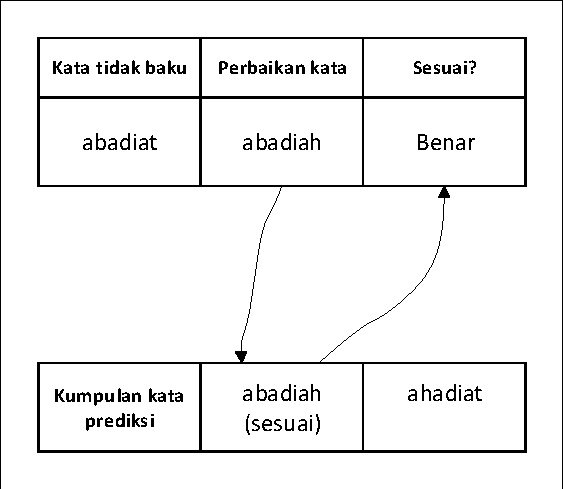
\includegraphics[width=0.6\textwidth, trim=2 2 2 2, clip]{resources/4/skenario1_eg.pdf}
	\caption{Contoh penilaian untuk pengujian skenario pertama}
	\label{fig:skenario1_eg}
\end{figure}

\subsection{Skenario Kedua: Melihat Seluruh Isi Kumpulan Kata}

Skenario kedua adalah penilaian dilakukan dengan melihat apakah terdapat perbaikan kata di dalam kumpulan kata prediksi. Contoh untuk skenario kedua dapat dilihat pada Gambar \ref{fig:skenario2_eg}. Seluruh kata dalam kumpulan kata prediksi diperiksa untuk menemukan salah satu kata yang sesuai dengan perbaikan kata. Jika ditemukan, maka kumpulan kata prediksi tersebut dianggap sesuai.
\begin{figure}[ht]
	\centering
	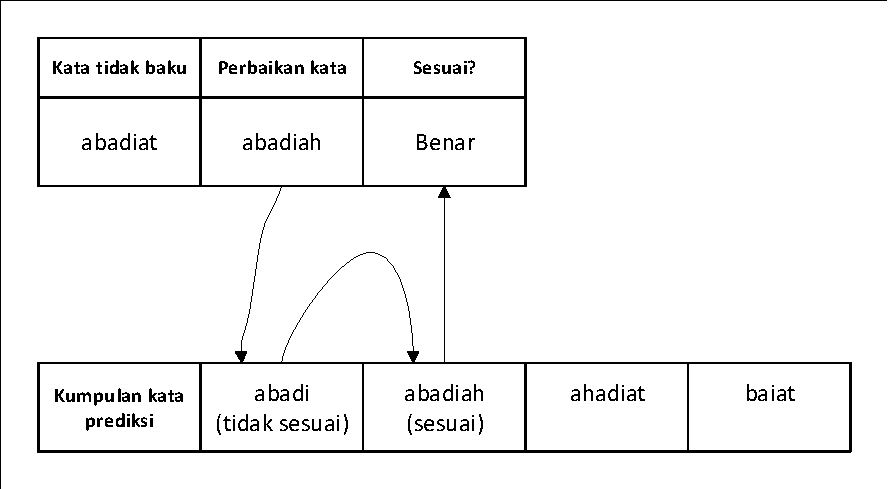
\includegraphics[width=0.8\textwidth, trim=2 2 2 2, clip]{resources/4/skenario2_eg.pdf}
	\caption{Contoh penilaian untuk pengujian skenario pertama}
	\label{fig:skenario2_eg}
\end{figure}

\section{Hasil Pengujian}

\subsection{Hasil Pengujian Skenario Pertama}

Hasil pengujian untuk skenario pengujian ditunjukkan pada Tabel \ref{tbl:result_1}. Hasil pengujian menunjukkan bahwa metode normalisasi yang diajukan mengungguli metode normalisasi \parencite{saragih2017normalisasi} dengan selisih akurasi sebesar 8,34 persen. Meskipun begitu, hasil akurasi pengujian untuk kedua metode masih menunjukkan angka di bawah 50 persen. Hal tersebut disebabkan oleh perbaikan kata uji bukan merupakan kata yang berada dalam urutan pertama kumpulan kata prediksi. Hal tersebut berarti perbaikan kata uji bukan merupakan kata yang sering digunakan dalam korpus Kompas. Sebagai contoh, perbaikan kata "\textit{asem}" seharusnya adalah "asam", namun dalam metode normalisasi usulan, kata "\textit{asem}" diidentifikasi sebagai "aset" yang mana "aset" adalah kata yang berada pada urutan pertama dalam kumpulan kata prediksi. Setelah melihat isi kumpulan kata prediksi, ternyata kata "asam" terdapat dalam kumpulan kata tersebut.
\begin{table}[ht]
    \captionsetup{justification=justified,singlelinecheck=false}
    \caption{Hasil akurasi untuk pengujian kedua metode normalisasi dalam skenario pertama}
    \label{tbl:result_1}
    \centering
    \begin{tabularx}{\textwidth}{|X|c|c|c|}
        \hline
        \multicolumn{1}{|Y|}{\textbf{Metode}} & \textbf{Jumlah kata benar} & \textbf{Akurasi} \\ \hline
        Metode Normalisasi \parencite{saragih2017normalisasi} dalam Skenario Pertama & 622 & 23,94\% \\ \hline
        Metode Normalisasi Usulan dalam Skenario Pertama & 774 & 32,28\% \\ \hline
    \end{tabularx}
\end{table}

Untuk melihat adanya kata perbaikan yang masuk ke dalam kumpulan kata dengan jarak perubahan minimum, diperlukan skenario baru, yaitu dengan modifikasi algoritme penilaian pada kedua metode normalisasi (skenario kedua). Gambar \ref{fig:skenario_side_to_side} menunjukkan perbedaan antara skenario pertama dengan skenario kedua. Jika skenario pertama hanya memeriksa urutan pertama dari kumpulan kata prediksi, skenario kedua memeriksa seluruh kumpulan kata prediksi hingga ditemukan kata yang sesuai dengan perbaikan kata.
\begin{figure}[ht]
	\centering
	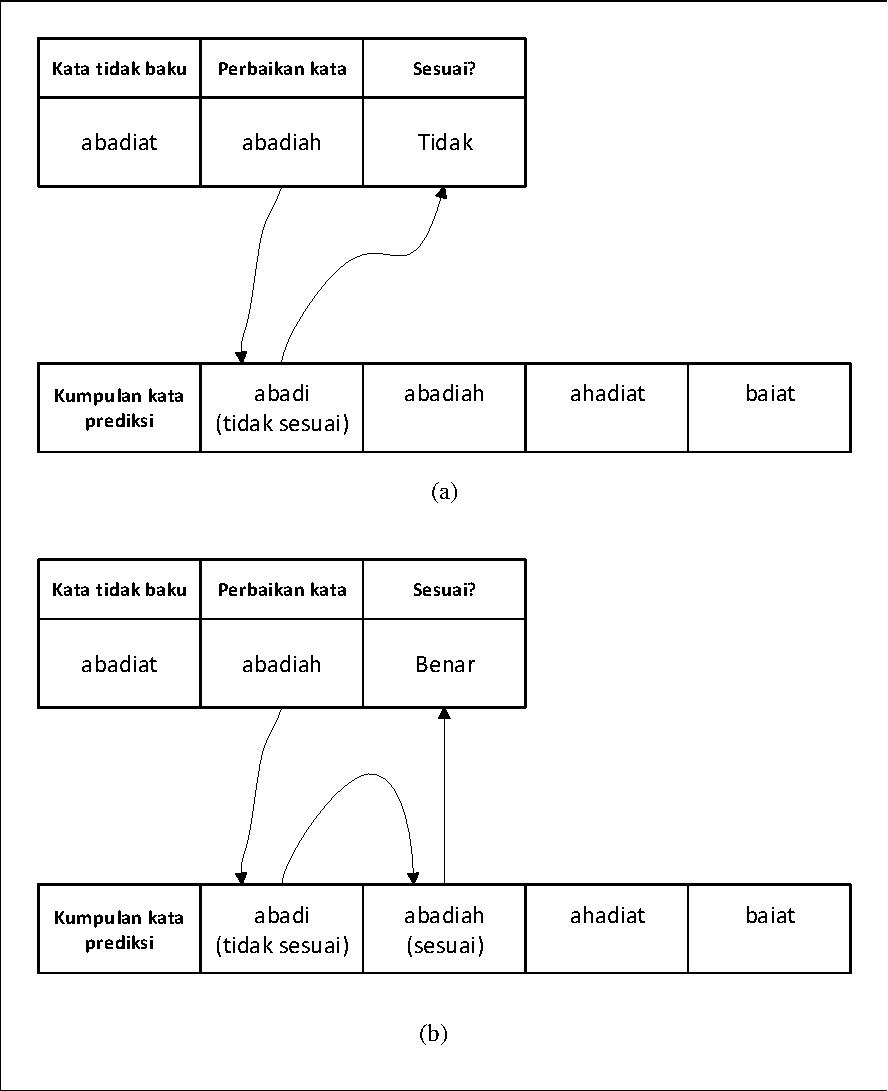
\includegraphics[width=0.5\textwidth, trim=2 2 2 2, clip]{resources/4/skenario_side_to_side.pdf}
	\caption{Perbedaan antara (a) skenario pertama, dan (b) skenario kedua}
	\label{fig:skenario_side_to_side}
\end{figure}

\subsection{Hasil Pengujian Skenario Kedua}

Hasil pengujian untuk skenario kedua ditunjukkan pada Tabel \ref{tbl:result_2}. Hasil pengujian tersebut menunjukkan peningkatan yang signifikan untuk selisih antara kedua metode, yaitu 18,89 persen. Hasil akurasi untuk metode normalisasi usulan masih mengungguli metode normalisasi \parencite{saragih2017normalisasi}. Namun, persentase akurasi belum menyentuh angka 100 persen.
\begin{table}[ht]
    \captionsetup{justification=justified,singlelinecheck=false}
    \caption{Hasil akurasi untuk pengujian kedua metode normalisasi dalam skenario kedua}
    \label{tbl:result_2}
    \centering
    \begin{tabularx}{\textwidth}{|X|c|c|c|}
        \hline
        \multicolumn{1}{|Y|}{\textbf{Metode}} & \textbf{Jumlah kata benar} & \textbf{Akurasi} \\ \hline
        Metode Normalisasi \parencite{saragih2017normalisasi} dalam Skenario Kedua & 1233 & 51,42\% \\ \hline
        Metode Normalisasi Usulan dalam Skenario Kedua & 1686 & 70,31\% \\ \hline
    \end{tabularx}
\end{table}

Hal tersebut dapat disebabkan oleh jarak perubahan antara kata tidak baku dan perbaikan kata uji tidak termasuk dalam kumpulan kata dengan  jarak perubahan minimum. Sebagai contoh, kata "\textit{telepa}" merupakan kata tidak baku dari kata "telap" dan jarak perubahan antara kedua kata adalah 3 dengan jarak LCS dan 2 dengan jarak Levenshtein. Namun, kedua metode normalisasi dapat menemukan kumpulan kata prediksi yang memiliki jarak perubahan yang lebih kecil dibandingkan jarak perubahan antara "\textit{telepa}" dan "telap" sehingga kata "telap" tidak dapat ditemukan.

Hasil pengujian tersebut menunjukkan bahwa masalah yang terjadi jika perbaikan kata uji telah diselesaikan, jika algoritme dalam metode normalisasi dapat melhat seluruh kata yang terkandung pada kumpulan kata prediksi. Namun, algoritme tersebut hanya dapat melihat kumpulan kata. Algoritme tidak dapat menentukan kata yang tepat digunakan, jika algoritme ingin diterapkan dalam sistem \textit{voice assistant}. Untuk penerapan dalam sistem \textit{voice assistant}, metode normalisasi juga harus dapat menentukan kata dalam kumpulan kata prediksi yang tepat digunakan.